\documentclass{standalone}

\usepackage{tikz}

\usetikzlibrary{patterns}
\usetikzlibrary{circuits.ee.IEC}

\begin{document}

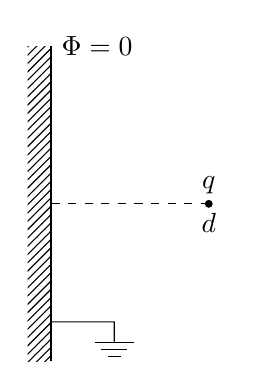
\begin{tikzpicture}[circuit ee IEC]
    \fill[pattern=north east lines](-.3, 0)rectangle(0, 4);
    \draw[thick](0, 0)--(0, 4)node[right]{$\Phi=0$};
    \draw (0, 0.5) to (0.8, 0.5) to [ground={at end}] (0.8, 0.15);
    \draw[dashed](0, 2)--(2, 2)node[below]{$d$};
    \fill[black](2, 2)circle(.05)node[above]{$q$};
\end{tikzpicture}\qquad
\begin{tikzpicture}
    \draw[dashed](0, 0)--(0, 4)node[right]{$\Phi=0$};
    \draw[dashed](-2, 2)--(2, 2);
    \fill[black](2, 2)circle(.05)node[above]{$q$};
    \fill[black](-2, 2)circle(.05)node[above]{$q'$};
\end{tikzpicture}
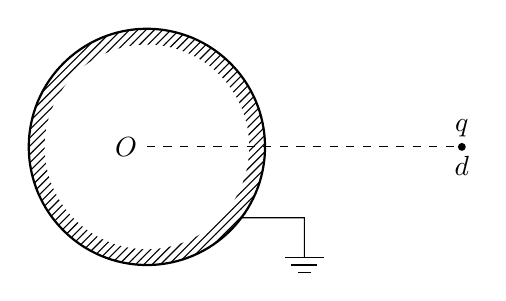
\begin{tikzpicture}[circuit ee IEC]
    \fill[even odd rule, pattern=north east lines](0, 0)circle(1.5)(0, 0)circle(1.3);
    \draw[thick](0, 0)circle(1.5);
    \draw (1.2, -.9) to (2, -.9) to [ground={at end}] (2, -1.5);
    \draw[dashed](0, 0)node[left]{$O$}--(4, 0);
    \fill[black](4, 0)circle(.05)node[below]{$d$}node[above]{$q$};
\end{tikzpicture}\\
\begin{tikzpicture}
    \draw[dashed](0, 0)circle(1.5);
    \draw[dashed](0, 0)node[left]{$O$}--(4, 0);
    \fill[black](4, 0)circle(.05)node[below]{$d$}node[above]{$q$};
    \fill[black](.5625, 0)circle(.05)node[below]{$d'$}node[above]{$q'$};
\end{tikzpicture}

\end{document}
